\chapter{การวิเคราะห์เชิงมาร์คอฟ (Markov Analysis)}

\section*{โจทย์ธุรกิจ}
\textbf{สถานการณ์ต้นบท: ความภักดีของลูกค้า (Customer Loyalty)}

หลังจากผ่านสถานการณ์ความไม่แน่นอนของตลาดและการตัดสินใจเรื่องกลยุทธ์การผลิตแล้ว  
ฝ่ายการตลาดของบริษัท ABC Furniture สังเกตเห็นปรากฏการณ์สำคัญที่กำลังส่งผลต่อผลประกอบการของบริษัท นั่นคือเรื่องของ \textbf{“การรักษาฐานลูกค้าจากบริการหลังการขาย”}

คุณสมชายและฝ่ายการตลาดพบข้อมูลที่น่าสนใจว่า ในแต่ละไตรมาส ลูกค้าของบริษัทมีแนวโน้มที่จะเปลี่ยนแปลงพฤติกรรมในการใช้บริการหลังการขายดังนี้:

\begin{itemize}
    \item ลูกค้าบางส่วนเป็น \textbf{ลูกค้าประจำ (Loyal Customers)} ที่ใช้บริการต่อเนื่องทุกไตรมาส
    \item ลูกค้าบางส่วนเป็น \textbf{ลูกค้าเปลี่ยนใจง่าย (Occasional Customers)} ที่ใช้บริการบ้างไม่ใช้บริการบ้าง
    \item ลูกค้าบางส่วนเป็น \textbf{ลูกค้าที่หายไป (Lost Customers)} ซึ่งหยุดใช้บริการจากบริษัท
\end{itemize}

ฝ่ายการตลาดต้องการวิเคราะห์ว่า ในแต่ละไตรมาสนั้น ลูกค้าจะเปลี่ยนแปลงสถานะจากกลุ่มหนึ่งไปอีกกลุ่มหนึ่งอย่างไร  
เพื่อที่จะได้วางแผนกลยุทธ์การตลาดและการบริหารความสัมพันธ์กับลูกค้า (CRM) ให้เหมาะสม

\vspace{0.5em}
\noindent
\textbf{อีเมลจากคุณสมชาย:}
\begin{tcolorbox}[colback=white!100!white, colframe=black!80!white,
  title=ข้อความ,
  fonttitle=\bfseries,
  sharp corners=southwest,
  boxrule=0.8pt,
  left=1mm, right=1mm, top=1mm, bottom=1mm,
]
\emph{
``ในช่วงไตรมาสที่ผ่านมา เราเริ่มสังเกตเห็นว่าฐานลูกค้าของเราเปลี่ยนแปลงเร็วมาก  
มีลูกค้าประจำหลายรายที่กลายเป็นลูกค้าเปลี่ยนใจง่าย  
และลูกค้ากลุ่มเปลี่ยนใจง่ายจำนวนไม่น้อยที่หยุดใช้บริการเราไปเลย  
แต่ในทางกลับกัน ก็ยังมีลูกค้าใหม่ๆ ที่เปลี่ยนจากลูกค้าเปลี่ยนใจง่ายมาเป็นลูกค้าประจำได้ด้วย  
เราอยากวิเคราะห์ให้ลึกกว่านี้ว่าการเปลี่ยนสถานะของลูกค้าเกิดขึ้นในลักษณะไหน  
เพื่อช่วยให้เราออกแบบกลยุทธ์รักษาฐานลูกค้าได้ดีขึ้นครับ"}
\end{tcolorbox}

\vspace{1em}
\noindent
\textbf{คำถามชวนคิดก่อนเรียน:}
\begin{enumerate}
    \item จากสถานการณ์ที่คุณสมชายเล่าให้ฟัง บริษัท ABC Furniture กำลังเจอกับปัญหาลักษณะใด?
    \item คุณคิดว่าการเปลี่ยนแปลงพฤติกรรมของลูกค้าในแต่ละไตรมาสเป็นเรื่องที่วิเคราะห์ได้อย่างไร?
    \item หากคุณจะสร้างแบบจำลองเพื่อวิเคราะห์พฤติกรรมลูกค้า คุณควรเก็บข้อมูลลักษณะใดบ้าง?
    \item สถานการณ์เช่นนี้ เหตุใดบริษัทจึงควรสนใจเรื่อง “การรักษาฐานลูกค้า” มากกว่าการหาลูกค้าใหม่เพียงอย่างเดียว?
    \item คุณคิดว่าการเปลี่ยนจากลูกค้าประจำไปเป็นลูกค้าเปลี่ยนใจง่าย หรือไปเป็นลูกค้าหายไป มีความสำคัญต่างกันหรือไม่ อย่างไร?
\end{enumerate}

\newpage
\section{ลักษณะของปัญหาที่ใช้ตัวแบบมาร์คอฟแก้ปัญหา}
\begin{itemize}
    \item ตัวแบบมาร์คอฟจะพิจารณาถึงความไม่แน่นอนของการเปลี่ยนสถานะในอนาคตโดยอ้างอิงจากสถานะในปัจจุบัน
    \item เพราะฉะนั้นปัญหาที่จะใช้ตัวแบบมาร์คอฟต้องสามารถแจกจางสถานะ (state) ขาดออกจากกันได้ โดยแต่ละตัวอย่างจะต้องอยู่ในสถานะใดสถานะหนึ่งและเพียงสถานะเดียวเท่านั้น
    \item ต้องมีข้อมูลเกี่ยวกับการแจกแจงความน่าจะเป็นหรืออัตราส่วนของแต่ละสถานะในปัจจุบัน
    \item ต้องทราบข้อมูลเรื่องความน่าจะเป็นของการเปลี่ยนสถานะ (transition probability)
\end{itemize}

\begin{example}
    {Warm-up ความน่าจะเป็นสำหรับ Markov (ต้องใช้ความรู้เรื่อง conditional probability)}{}
    ในเหตุการณ์สมมติที่มีสถานะ 3 สถานะ สมมติเป็น $s_1, s_2, s_3$ โดยเราทราบความน่าจะเป็นของการเปลี่ยนสถานะจากสถานะ $s_1, s_2, s_3$ มาเป็นสถานะ $s_1$ ในระยะเวลา 1 เดือนมีค่าเป็น $0.10, 0.90, 0.05$ ตามลำดับ โดยในปัจจุบันเราทราบว่ามีจำนวนคนที่มีสถานะเป็น $s_1, s_2, s_3$ อยู่เป็น $30,75,40$ คนตามลำดับ
    \begin{itemize}
        \item ทำไมความน่าจะเป็นของการเปลี่ยนสถานะจากสถานะ $s_1, s_2, s_3$ มาเป็นสถานะ $s_1$ ถึงรวมกันได้ไม่เท่ากับ 1
        \item จงหาจำนวนคนในสถานะ $s_1$ ใน 1 เดือนข้างหน้า
    \end{itemize}
\end{example}
\newpage
\section{คณิตศาสตร์สำหรับตัวแบบมาร์คอฟ}
จากตัวอย่างที่ผ่านมานั้น เป็นตัวอย่างที่ได้ทำให้เห็นแนวคิดการคิดแบบความน่าจะเป็นว่าการวิเคราะห์การเปลี่ยนสถานะนั้น จริงๆ แล้วก็คือการหาความน่าจะเป็นของ 2 เหตุการณ์ต่อเนื่องกันในรูปแบบของความน่าจะเป็นแบบมีเงื่อนไข (Conditional Probability) และคุณสมบัติความน่าจะเป็นรวม (Total probability)
\begin{align*}
    \text{จำนวน}&\text{คนในสถานะ $s_1$ ในเวลาถัดมา}\\ 
            &= \text{จำนวนคนทั้งหมด}\times P(\text{สุ่มหยิบได้คน $s_1$ ในเวลาถัดมา})\\
            &= N \cdot P(X^{(2)} = s_1)\\
            &= N\cdot\left(P(X^{(1)} = s_1 \wedge X^{(2)} = s_1) + P(X^{(1)} = s_2 \wedge X^{(2)} = s_1) + P(X^{(1)} = s_3 \wedge X^{(2)} = s_1)  \right)\\
            &= N\cdot\bigl[ P(X^{(1)} = s_1)P(X^{(2)} = s_1 | X^{(1)} = s_1) \\
            &\qquad\quad+ P(X^{(1)} = s_2)P(X^{(2)} = s_1 | X^{(1)} = s_2)\\
            &\qquad\quad+ P(X^{(1)} = s_3)P(X^{(2)} = s_1 | X^{(1)} = s_3) \bigr]\\
            &= N\cdot\bigl[ P(\text{สุ่มหยิบได้คน $s_1$ ในเวลาเริ่ม})P(\text{เปลี่ยนจาก $s_1$ ไปเป็น $s_1$}) \\
            &\qquad\quad+ P(\text{สุ่มหยิบได้คน $s_2$ ในเวลาเริ่ม})P(\text{เปลี่ยนจาก $s_2$ ไปเป็น $s_1$})\\
            &\qquad\quad+ P(\text{สุ่มหยิบได้คน $s_3$ ในเวลาเริ่ม})P(\text{เปลี่ยนจาก $s_3$ ไปเป็น $s_1$}) \bigr]\\
            &= (\text{จำนวนคน $s_1$ ในเวลาเริ่ม})P(\text{เปลี่ยนจาก $s_1$ ไปเป็น $s_1$}) \\
            &\qquad\quad+ (\text{จำนวนคน $s_1$ ในเวลาเริ่ม})P(\text{เปลี่ยนจาก $s_2$ ไปเป็น $s_1$})\\
            &\qquad\quad+ (\text{จำนวนคน $s_1$ ในเวลาเริ่ม})P(\text{เปลี่ยนจาก $s_3$ ไปเป็น $s_1$})
\end{align*}

ในทำนองเดียวกัน เราจึงได่ว่า
\begin{align*}
    \text{จำนวน}\text{คนในสถานะ $s_1$ ในเวลาถัดมา}
            &= (\text{จำนวนคน $s_1$ ในเวลาเริ่ม})P(\text{เปลี่ยนจาก $s_1$ ไปเป็น $s_1$}) \\
            &\quad+ (\text{จำนวนคน $s_2$ ในเวลาเริ่ม})P(\text{เปลี่ยนจาก $s_2$ ไปเป็น $s_1$})\\
            &\quad+ (\text{จำนวนคน $s_3$ ในเวลาเริ่ม})P(\text{เปลี่ยนจาก $s_3$ ไปเป็น $s_1$})\\
            ~\\
    \text{จำนวน}\text{คนในสถานะ $s_2$ ในเวลาถัดมา}
            &= (\text{จำนวนคน $s_1$ ในเวลาเริ่ม})P(\text{เปลี่ยนจาก $s_1$ ไปเป็น $s_2$}) \\
            &\quad+ (\text{จำนวนคน $s_2$ ในเวลาเริ่ม})P(\text{เปลี่ยนจาก $s_2$ ไปเป็น $s_2$})\\
            &\quad+ (\text{จำนวนคน $s_3$ ในเวลาเริ่ม})P(\text{เปลี่ยนจาก $s_3$ ไปเป็น $s_2$})\\
            ~\\
    \text{จำนวน}\text{คนในสถานะ $s_3$ ในเวลาถัดมา}
            &= (\text{จำนวนคน $s_1$ ในเวลาเริ่ม})P(\text{เปลี่ยนจาก $s_1$ ไปเป็น $s_3$}) \\
            &\quad+ (\text{จำนวนคน $s_2$ ในเวลาเริ่ม})P(\text{เปลี่ยนจาก $s_2$ ไปเป็น $s_3$})\\
            &\quad+ (\text{จำนวนคน $s_3$ ในเวลาเริ่ม})P(\text{เปลี่ยนจาก $s_3$ ไปเป็น $s_3$})
\end{align*}

เพื่อความสะดวกในการเขียนเป็นสัญลักษณ์เมทริกซ์ในส่วนถัดไป ขอกำหนดสัญลักษณ์ดังนี้
\begin{align*}
    N_i &= \text{จำนวนคนในสถานะ $s_i$ ในเวลาเริ่ม}\\
    N_i^{\prime} &= \text{จำนวนคนในสถานะ $s_i$ ในเวลาถัดมา}\\
    P_{ij} &= \text{ความน่าจะเป็นในการเปลี่ยนสถานะจาก $s_j$ มาเป็น $s_i$}
\end{align*}
ดังนั้น เราจึงได้ว่า
\begin{align*}
    N^{\prime}_1 &= N_1 P_{11} + N_2 P_{12} + N_3 P_{13}\\
    N^{\prime}_2 &= N_1 P_{21} + N_2 P_{22} + N_3 P_{23}\\
    N^{\prime}_3 &= N_1 P_{31} + N_2 P_{32} + N_3 P_{33}
\end{align*}
และเมื่อนำมาลองเขียนในรูปแบบเวกเตอร์แจกแจงจำนวนคน จะได้ว่า
\begin{align*}
    \vec{N}^{\prime} &= \begin{pmatrix}N^{\prime}_1 \\ N^{\prime}_2 \\ N^{\prime}_3\end{pmatrix}\\
                  &= \begin{pmatrix}
                  N_1 P_{11} + N_2 P_{12} + N_3 P_{13} \\ 
                  N_1 P_{21} + N_2 P_{22} + N_3 P_{23} \\ 
                  N_1 P_{31} + N_2 P_{32} + N_3 P_{33}\end{pmatrix}\\
                  &= \begin{bmatrix}P_{11} & P_{12} & P_{13} \\ 
                  P_{21} & P_{22} & P_{23} \\
                 P_{31} & P_{32} & P_{33} \end{bmatrix}\begin{pmatrix}N_1 \\ N_2 \\ N_3\end{pmatrix}\\
    \vec{N}^{\prime} &= \begin{bmatrix}P_{11} & P_{12} & P_{13} \\ 
                  P_{21} & P_{22} & P_{23} \\
                 P_{31} & P_{32} & P_{33} \end{bmatrix}\vec{N}
\end{align*}

\begin{definition}
    {Transition Matrix}{}
    เมทริกซ์การเปลี่ยนสถานะ (transition matrix) คือเมทริกซ์ที่ลำดับของแถวและหลักของเมทริกซ์สอดคล้องกับลำดับสถานะ $s_1,\dots,s_n$ โดยที่สมาชิกในตำแหน่งที่ $ij$ คือค่าความน่าจะเป็นของการเปลี่ยนจากสถานะ $j$ มาเป็นสถานะ $i$
\end{definition}

\begin{property}
    {การหาจำนวนคนในแต่ละสถานะในช่วงเวลาถัดไป}{}
    กำหนดให้ $N_t$ แทนเวกเตอร์ของจำนวนคนในแต่ละสถานะ โดยที่ลำดับของสถานะเป็น $s_1,\dots,s_n$ และให้ $P$ คือเมทริกซ์เปลี่ยนสถานะที่มีลำดับของสถานะเดียวกันกับลำดับสถานะของเวกเตอร์ $N_t$ จะได้ว่า
    \[
    N_{t+1} = P N_t
    \]

    เพราะฉะนั้น จะได้โดยง่ายว่า
    \[
    N_{t+k} = P^k N_t
    \]
    ทั้งนี้ เราอาจจะเปลี่ยนไปใช้เวกเตอร์ที่แสดงความน่าจะเป็นแทนเวกเตอร์จำนวนคนจริง ๆ ก็ได้
\end{property}
\newpage
\begin{example}
    {การคำนวณมาร์คอฟของโรงอาหาร}{canteenMarkov}
    โรงอาหารในบริษัทแห่งหนึ่งมีเมนูประจำร้าน 3 เมนู สมมติชื่อชุด A, B และ C โดยแต่ละเมนูมีการเตรียมวัตถุดิบที่แตกต่างกันออกไป ทางร้านจึงต้องการวางแผนอัตราส่วนของปริมาณของวัตถุดิบของอาหารแต่ละประเภทที่ต้องเก็บเข้าคลังไว้เป็นรายเดือน ดังนั้น ทางร้านจึงได้ทำการสำรวจพฤติกรรมการเปลี่ยนแปลงประเภทอาหารที่จะทานของพนักงานในบริษัทแห่งนั้น และได้ความน่าจะเป็นของการเปลี่ยนแปลงประเภทอาหารที่อยากทานใน 1 เดือนดังตารางด้านล่างนี้ (ให้สมมติว่าบริษัทไม่ได้มีการสมัครเข้าหรือลาออกบ่อย และในบริษัทมีร้านอาหารผูกขาดอยู่ร้านเดียว)
    \begin{center}
    \begin{tabular}{ll|lll|}
        \cline{3-5}
                                                                     &   & \multicolumn{3}{l|}{เมนูที่ทานเดือนนี้}                   \\ \cline{3-5} 
                                                                     &   & \multicolumn{1}{l|}{A}   & \multicolumn{1}{l|}{B}   & C   \\ \hline
        \multicolumn{1}{|l|}{\multirow{3}{*}{เมนูที่่ทานเดือนถัดไป}} & A & \multicolumn{1}{l|}{0.6} & \multicolumn{1}{l|}{0.6} & 0.2 \\ \cline{2-5} 
        \multicolumn{1}{|l|}{}                                       & B & \multicolumn{1}{l|}{0.3} & \multicolumn{1}{l|}{0.1} & 0.2 \\ \cline{2-5} 
        \multicolumn{1}{|l|}{}                                       & C & \multicolumn{1}{l|}{0.1} & \multicolumn{1}{l|}{0.3} & 0.6 \\ \hline
    \end{tabular}  
    \end{center}
    สมมติว่าในเดือนนี้มีปริมาณการทานอาหารเมนู A, B, C เป็นจำนวน 60 ครั้ง, 100 ครั้ง, 40 ครั้ง ตามลำดับ
    \begin{enumerate}
        \item จงหาว่าในเดือนถัดไปจะมีการทานอาหารในแต่ละเมนูกี่ครั้ง
        \item จงหาว่าในอีก 2 เดือนถัดไปจะมีการทานอาหารในแต่ละเมนูกี่ครั้ง
    \end{enumerate}
\end{example}

\newpage
\section{การวิเคราะห์สถานะคงที่่}
\begin{definition}
    {สถานะคงที่ (Steady State)}{}
    สถานะคงที่ของกระบวนการมาร์คอฟคือเวกเตอร์สถานะที่เมื่อผ่านขั้นตอนถัดไปแล้วมีสถานะคงเดิม (อัตราส่วนเท่าเดิม) กล่าวคือเวกเตอร์ $\vec{s}$ จะเป็นสถานะคงที่ของเมทริกซ์การเปลี่ยนสถานะ $P$ ก็ต่อเมื่อ
    \[
    P\vec{s} = \vec{s}
    \]
    \footnote{ในคณิตศาสตร์จะเรียกว่า $\vec{s}$ เป็น eigenvector ที่สอคคล้องกับ eigenvalue = 1 ของเมทริกซ์ $P$}ทั้งนี้เวกเตอร์ที่เป็นสเกลของเวกเตอร์สถานะคลที่ก็ยังคงเป็นสถานะคงที่เช่นกัน ดังนั้นในบางครั้งเราอาจจะระบุเพียงแค่เวกเตอร์ความน่าจะเป็น ณ สถานะคงที่ ซึ่งคือทุกสมาชิกในเวกเตอร์รวมกันได้ 1
\end{definition}

\begin{example}
    {เวกเตอร์สถานะคงที่}{}
    จงหาเวกเตอร์ความน่าจะเป็น ณ สถานะคงที่ของเมทริกซ์การเปลี่ยนสถานะของผู้รับบริการ $\begin{bmatrix}0.7 & 0.4 \\ 
                  0.3 & 0.6 \end{bmatrix}$
    และถ้าสมมติว่า ณ เวลานั้นมีผู้รับบริการทั้งหมดอยู่ 500 คน จะมีคนอยู่ในแต่ละสถานะกี่คน
\end{example}
\newpage

\begin{example}
    {มาร์คอฟของโรงอาหาร (ต่อ)}{}
    จากตัวอย่างสถานะการโรงอาหารในบริษัทในตัวอย่าง \ref{ex:canteenMarkov} จงหาว่าต้องมีอัตราส่วนของคนชอบเมนูอาหารใดเท่าไหร่บ้างถึงจะอยู่ในสภาวะที่ไม่ต้องเปลี่ยนแปลงปริมาณการเก็บวัตถุดิบในเดือนถัดไป
\end{example}
\newpage
\section{การคำนวณ Markov โดยใช้ Excel}
\newpage
\section{หัวข้อพิเศษ: การคูณเมทริกซ์กับเมทริกซ์ในมุมมองของมาร์คอฟ}
อย่างที่ได้กล่าวไปในหัวข้อที่ผ่าน ๆ มาว่าเราสามารถหาเวกเตอร์ความน่าจะเป็นของแต่ละสถานะ

\begin{exercise}{หาผลกำลังสองของเมทริกซ์ความน่าจะเปลี่ยนของการเปลี่ยนสถานะ}{quiz3}
	จงหาผลคูณของเมทริกซ์ได้ผลลัพธ์ดังนี้ (โจทย์ให้ผลลัพธ์การคูณมาแล้ว ดังนั้นไม่ต้องนั่งคูณด้วยตัวเอง แต่เราจะลองใช้ความรู้ Markov ช่วยหาผลคูณ และในข้อนี้เราจะไม่ได้หาผลคูณของทั้ง 9 ตัว เราจะยกตัวอย่างการหาผลคูณของแค่ 3 ตัวเท่านั้น)
	$$
	\begin{bmatrix}
		0.6 & 0.6 & 0.2 \\
		0.3 & 0.1 & 0.2 \\
		0.1 & 0.3 & 0.6 \\
	\end{bmatrix} \times
	\begin{bmatrix}
		0.6 & 0.6 & 0.2 \\
		0.3 & 0.1 & 0.2 \\
		0.1 & 0.3 & 0.6 \\
	\end{bmatrix}
	=
	\begin{bmatrix}
		0.56 & 0.48 & 0.36 \\
		0.23 & 0.25 & 0.20 \\
		0.21 & 0.27 & 0.44 \\
	\end{bmatrix}
	$$
\end{exercise}

เริ่มจากเขียนแผนภาพการเปลี่ยนสถานะกันก่อน โดยโจทย์คือให้\underline{\textbf{เขียนค่าความน่าจะเป็นลงไปบนเส้นการเปลี่ยนสถานะ}}
\begin{center}
	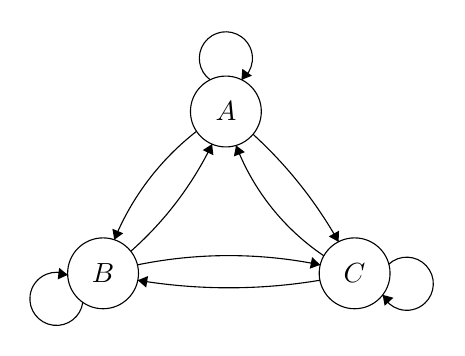
\begin{tikzpicture}[scale=0.15]
		\tikzstyle{every node}+=[inner sep=0pt]
		\draw [black] (23.7,-25.4) circle (3);
		\draw (23.7,-25.4) node {$A$};
		\draw [black] (13.3,-39.1) circle (3);
		\draw (13.3,-39.1) node {$B$};
		\draw [black] (34.6,-39.1) circle (3);
		\draw (34.6,-39.1) node {$C$};
		\draw [black] (14.249,-36.256) arc (157.70826:127.88572:22.39);
		\fill [black] (14.25,-36.26) -- (15.01,-35.71) -- (14.09,-35.33);
		\draw [black] (22.535,-28.163) arc (-25.83943:-48.56659:28.903);
		\fill [black] (22.53,-28.16) -- (21.74,-28.67) -- (22.64,-29.1);
		\draw [black] (16.213,-38.384) arc (101.57892:78.42108:38.549);
		\fill [black] (31.69,-38.38) -- (31,-37.73) -- (30.8,-38.71);
		\draw [black] (31.659,-39.688) arc (-80.52759:-99.47241:46.841);
		\fill [black] (16.24,-39.69) -- (16.95,-40.31) -- (17.11,-39.33);
		\draw [black] (25.997,-27.328) arc (47.64144:29.37151:36.624);
		\fill [black] (33.24,-36.43) -- (33.28,-35.49) -- (32.41,-35.98);
		\draw [black] (31.995,-37.618) arc (-123.95959:-159.02746:19.823);
		\fill [black] (24.56,-28.27) -- (24.38,-29.2) -- (25.31,-28.84);
		\draw [black] (22.377,-22.72) arc (234:-54:2.25);
		\fill [black] (25.02,-22.72) -- (25.9,-22.37) -- (25.09,-21.78);
		\draw [black] (37.487,-38.329) arc (132.69007:-155.30993:2.25);
		\fill [black] (36.97,-40.92) -- (37.14,-41.85) -- (37.88,-41.17);
		\draw [black] (11.585,-41.547) arc (-7.29476:-295.29476:2.25);
		\fill [black] (10.31,-39.23) -- (9.58,-38.63) -- (9.46,-39.62);
	\end{tikzpicture}
\end{center}


จากที่เรียนมาในห้อง เราทราบกันอยู่แล้วว่าความหมายของการนำเมทริกซ์การเปลี่ยนสถานะ 1 ขั้นมาคูณกัน จะได้ผลออกมาเป็นเมทริกซ์การเปลี่ยนสถานะข้าม 2 ขั้น (เช่นเปลี่ยนจากขั้นที่ 1 ไปขั้นที่ 3)
ดังนั้น ถ้าเราอยากหาผลคูณของเมทริกซ์การเปลี่ยนสถานะ สิ่งที่ต้องทำคือหาความน่าจะเป็นในการเดินข้าม 2 ขั้นทุกรูปแบบที่เป็นไปได้

\subsubsection*{การเปลี่ยนสถานะจาก A ในขั้นที่ 1 ไป A ในขั้นที่ 3}
วาดแผนภาพด้านล่าง โจทย์คือ \underline{\textbf{จงเขียนค่าความน่าจะเป็นของการย้ายสถานะของแต่ละเส้น (มี 6 เส้น)}}
\begin{center}
	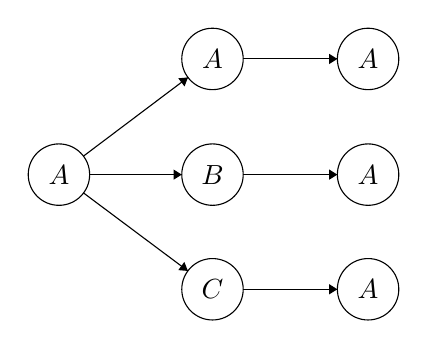
\begin{tikzpicture}[scale=0.13]
		\tikzstyle{every node}+=[inner sep=0pt]
		\draw [black] (11,-31.3) circle (3);
		\draw (11,-31.3) node {$A$};
		\draw [black] (26,-31.3) circle (3);
		\draw (26,-31.3) node {$B$};
		\draw [black] (26,-42.5) circle (3);
		\draw (26,-42.5) node {$C$};
		\draw [black] (26,-20) circle (3);
		\draw (26,-20) node {$A$};
		\draw [black] (41.2,-20) circle (3);
		\draw (41.2,-20) node {$A$};
		\draw [black] (41.2,-31.3) circle (3);
		\draw (41.2,-31.3) node {$A$};
		\draw [black] (41.2,-42.5) circle (3);
		\draw (41.2,-42.5) node {$A$};
		\draw [black] (13.4,-29.49) -- (23.6,-21.81);
		\fill [black] (23.6,-21.81) -- (22.66,-21.89) -- (23.27,-22.69);
		\draw [black] (14,-31.3) -- (23,-31.3);
		\fill [black] (23,-31.3) -- (22.2,-30.8) -- (22.2,-31.8);
		\draw [black] (13.4,-33.09) -- (23.6,-40.71);
		\fill [black] (23.6,-40.71) -- (23.25,-39.83) -- (22.66,-40.63);
		\draw [black] (29,-20) -- (38.2,-20);
		\fill [black] (38.2,-20) -- (37.4,-19.5) -- (37.4,-20.5);
		\draw [black] (29,-31.3) -- (38.2,-31.3);
		\fill [black] (38.2,-31.3) -- (37.4,-30.8) -- (37.4,-31.8);
		\draw [black] (29,-42.5) -- (38.2,-42.5);
		\fill [black] (38.2,-42.5) -- (37.4,-42) -- (37.4,-43);
	\end{tikzpicture}
\end{center}

ด้วยความรู้ในเรื่องความน่าจะเป็น เราจะได้ว่าความน่าจะเป็นรวมของการย้ายสถานะจาก A ข้ามไป A ใน 2 ขั้นถัดไปหาได้จากกฏการคูณและการบวกจากแผนภาพต้นไม้ดังกล่าว โดยที่
\begin{itemize}
	\item เส้นต่อกัน ให้นำค่าความน่าจะเป็นของเส้นมาคูณกัน
	\item หลังจากคิดผลคูณค่าความน่าจะเป็นของแต่ละกิ่งเรียบร้อยแล้ว ให้นำมาบวกกัน
\end{itemize}
เพราะฉะนั้น เราจะได้ว่าความน่าจะเป็นของการเปลี่ยนสถานะจาก A ข้ามไป A ใน 2 ขั้นถัดไปมีค่าเท่ากับ
$$
P(A\rightarrow_2A) = \left(\blank{1cm}\times\blank{1cm}\right) + \left(\blank{1cm}\times\blank{1cm}\right) + \left(\blank{1cm}\times\blank{1cm}\right) = 0.56
$$
ซึ่งมีผลลัพธ์เท่ากับสมาชิกในแถวที่ 1 หลักที่ 1 ที่แทนความน่าจะเป็นของการเปลี่ยนจาก A ไป A ในเมทริกซ์ผลลัพธ์
\subsubsection*{การเปลี่ยนสถานะจาก A ในขั้นที่ 1 ไป B ในขั้นที่ 3}
วาดแผนภาพด้านล่าง โจทย์คือ \underline{\textbf{จงเขียนค่าความน่าจะเป็นของการย้ายสถานะของแต่ละเส้น (มี 6 เส้น)}}
\begin{center}
	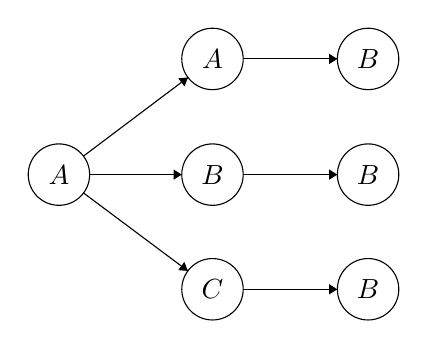
\begin{tikzpicture}[scale=0.13]
		\tikzstyle{every node}+=[inner sep=0pt]
		\draw [black] (11,-31.3) circle (3);
		\draw (11,-31.3) node {$A$};
		\draw [black] (26,-31.3) circle (3);
		\draw (26,-31.3) node {$B$};
		\draw [black] (26,-42.5) circle (3);
		\draw (26,-42.5) node {$C$};
		\draw [black] (26,-20) circle (3);
		\draw (26,-20) node {$A$};
		\draw [black] (41.2,-20) circle (3);
		\draw (41.2,-20) node {$B$};
		\draw [black] (41.2,-31.3) circle (3);
		\draw (41.2,-31.3) node {$B$};
		\draw [black] (41.2,-42.5) circle (3);
		\draw (41.2,-42.5) node {$B$};
		\draw [black] (13.4,-29.49) -- (23.6,-21.81);
		\fill [black] (23.6,-21.81) -- (22.66,-21.89) -- (23.27,-22.69);
		\draw [black] (14,-31.3) -- (23,-31.3);
		\fill [black] (23,-31.3) -- (22.2,-30.8) -- (22.2,-31.8);
		\draw [black] (13.4,-33.09) -- (23.6,-40.71);
		\fill [black] (23.6,-40.71) -- (23.25,-39.83) -- (22.66,-40.63);
		\draw [black] (29,-20) -- (38.2,-20);
		\fill [black] (38.2,-20) -- (37.4,-19.5) -- (37.4,-20.5);
		\draw [black] (29,-31.3) -- (38.2,-31.3);
		\fill [black] (38.2,-31.3) -- (37.4,-30.8) -- (37.4,-31.8);
		\draw [black] (29,-42.5) -- (38.2,-42.5);
		\fill [black] (38.2,-42.5) -- (37.4,-42) -- (37.4,-43);
	\end{tikzpicture}
\end{center}

เพราะฉะนั้น เราจะได้ว่าความน่าจะเป็นของการเปลี่ยนสถานะจาก A ข้ามไป B ใน 2 ขั้นถัดไปมีค่าเท่ากับ
$$
P(A\rightarrow_2B) = \left(\blank{1cm}\times\blank{1cm}\right) + \left(\blank{1cm}\times\blank{1cm}\right) + \left(\blank{1cm}\times\blank{1cm}\right) = \blank{1cm}
$$